\subsection{NHIỆT DUNG RIÊNG}
\newghichu{
\begin{itemize}
\item \textbf{Nhiệt dung riêng} của một chất là nhiệt lượng cần truyền cho 1 kg chất đó để làm cho nhiệt độ của nó tăng thêm 1 độ ($1^\circ C$ hoặc 1 K).
\item Kí hiệu: c
\item Đơn vị: $J/kg.K$
\end{itemize}
}
\begin{note}
Nhiệt dung riêng của nhôm là 880 J/kg.K nghĩa là nhiệt lượng cần truyền cho 1 kg nhôm để làm nhiệt độ của nó tăng thêm 1 K là 880 J. 
\end{note}
\begin{bang}[ tabularx=X|X]{Nhiệt dung riêng của một số chất}
\text { Chất } & \text { Nhiệt dung riêng } ($J/kg.K$)\\\hline 
Nhôm & 880 \\ \hline  
Thủy ngân & 140 \\\hline  
Đồng & 380 \\\hline  
Chì & 126 \\ \hline  
Nước biển & 3950 \\ \hline  
Nước & 4180\\ \hline  
Rượu & 2500\\ \hline  
\end{bang}
\subsection{HỆ THỨC TÍNH NHIỆT LƯỢNG TRONG QUÁ TRÌNH TRUYỀN NHIỆT ĐỂ LÀM THAY ĐỔI NHIỆT ĐỘ CỦA VẬT}
\newghichu{Độ lớn của nhiệt lượng cần cung cấp cho vật để làm tăng nhiệt độ của nó phụ thuộc vào: khối lượng của vật; độ tăng nhiệt độ và tính chất của chất làm vật}
\begin{align*}
\boder{Q=mc\Delta t=mc(t_2-t_1)}
\quad \begin{cases}
\ct{c: nhiệt dung riêng (J/kg.K) của chất}\\
\ct{m: khối lượng của vật (kg)}\\
t_1\ct{: nhiệt độ ban đầu của vật}\\
t_2\ct{: nhiệt độ lúc sau của vật}
\end{cases}
\end{align*}
\begin{note}
$Q>0$: Vật thu nhiệt\\
$Q<0$: Vật tỏa nhiệt  
\end{note}
\subsection{ĐIỀU KIỆN CÂN BẰNG NHIỆT} 
\newghichu{
Khi hệ cô lập về nhiệt ở trạng thái cân bằng nhiệt, tổng nhiệt lượng trao đổi của các vật trong hệ bằng không.
}
\begin{align*}
\boder{Q_1+Q_2+...+Q_n=0}
\quad 
\begin{cases}
Q_1=m_1.c_1.(t-t_1);\ Q_2=m_2.c_2.(t-t_2),...\\
t_1,\ t_2,... \ct{là nhiệt độ ban đầu của các vật}\\
t\ \ct{là nhiệt độ của các vật ở trạng thái cân bằng nhiệt}
\end{cases}
\end{align*}
\subsection{ỨNG DỤNG NHIỆT DUNG RIÊNG}
Nhiệt dung riêng là thông tin quan trọng được dùng khi lựa chọn vật liệu cho các hệ thống làm mát, sưởi ấm,…
\begin{center}
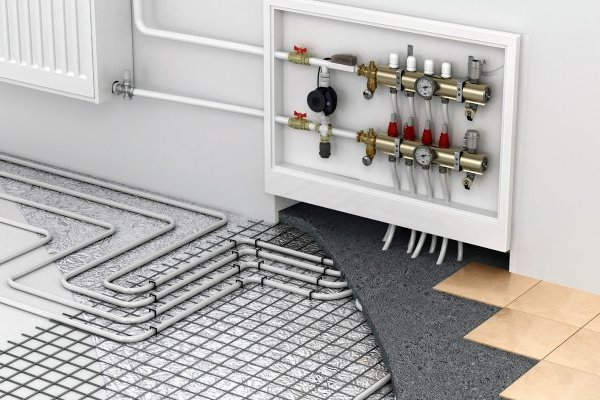
\includegraphics[width=8cm]{Images/suoisan}
\begin{center}
\textit{Hệ thống sưởi ấm sàn}
\end{center}	
\end{center}
%\subsection*{II. Thí nghiệm xác định nhiệt dung riêng của nước}
%\setcounter{paragraph}{0}
%\subsubsection{Phương án 1}
%\begin{itemize}
%	\item Dụng cụ
%
%immini{\begin{itemize}
%	\item Biến thế nguồn (1).
%	\item Bộ đo công suất nguồn điện (oát kế), đồng hồ bấm giây (2).
%	\item Nhiệt kế điện tử (3).
%	\item Nhiệt lượng kế (4).
%	\item Cân điện tử (5).
%\end{itemize}}{includegraphics[width=4cm]{Images/tn2}}
%\item Tiến hành thí nghiệm
%\begin{center}
%includegraphics[width=8cm]{Images/tn3}
%\end{center}
%	\begin{itemize}
%	\item Đổ một lượng nước vào bình nhiệt lượng kế sao cho toàn bộ dây điên trở chìm trong nước.
%	\item Xác định khối lượng nước trong bình.
%	\item Bật biến áp nguồn, khoáy liên tục để nước nóng đều. 
%	\item Cứ sau mỗi khoảng 1 phút, đọc số chỉ công suất đun $\mathcal{P}$ của oát kế, nhiệt độ từ nhiệt kế rồi điền vào bảng theo mẫu sau:
%	\begin{bang}[tabularx=X|X|X|X]{Bảng số liệu mẫu kết quả đo nhiệt dung riêng của nước}
%		Lần đo&Nhiệt độ $t\ (^\circ C)$&Thời gian $\tau\ (s)$&Công suất $\mathcal{P}\ (W)$\\\hline 
%		1&&&\\\hline 
%		2&&&\\\hline 
%		3&&&\\\hline 
%		4&&&\\\hline 
%		5&&&\\\hline 
%	\end{bang}
%	\item Vẽ đồ thị nhiệt độ t theo thời gian $\tau$.
%	\item[] 
%%	\begin{center}
%\centering{includegraphics[width=4cm]{Images/dt1}}
%%	\begin{center}
%	\item[]
%	\item Chọn hai điểm M, N trên đồ thị, xác định các giá trị thời gian $\tau_M,\ \tau_N$ và nhiệt độ $t_M,\ t_N$. 
%	\item Tính nhiệt dung riêng của nước theo hệ thức: 
%	\begin{align*}
%		c_{H_2O}=\dfrac{Q}{m\Delta t}=\dfrac{\overline{\mathcal{P}}\Delta \tau}{m.\Delta t}
%	\end{align*}
%		\begin{itemize}
%		\item m (kg): khối lượng của nước
%		\item $\Delta t=t_M-t_M\ (^\circ C)$: Độ tăng nhiệt độ của nước
%		\item $\overline{\mathcal{P}}$ (W): Công suất đun trung bình
%		\item $\Delta \tau=\tau_M-\tau_M\ (s)$: Thời gian đun
%\end{itemize}	
%\end{itemize}	
%\end{itemize}
%\subsubsection{Phương án 2}
%\begin{itemize}
%	\item Dụng cụ
%	immini{\begin{itemize}
%		\item 1 biến thế nguồn (1)
%		\item 2 đồng hồ đo điện đa năng dùng làm vôn kế một chiều và ampe kế một chiều (2)
%		\item Dây nối (3)
%		\item 1 bình nhiệt lượng kế (có dây nung và que khuấy) (4)
%		\item 1 đồng hồ đo thời gian có chia độ chia nhỏ nhất 0,01 s (5)
%		\item 1 nhiệt kế có độ chia nhỏ nhất  $1^\circ C$ (6)
%		\item 1 chai nước nhiệt độ phòng (7)
%		\item 1 chiếc cân điện tử có độ chia nhỏ nhất  (8)
%		\item 1 công tắc điện từ (9)
%	\end{itemize}}{includegraphics[width=4cm]{Images/tn4}}
%	\item Tiến thành thí nghiệm
%		immini{\begin{itemize}
%		\item Cho một lượng nước có khối lượng $m_n$ và nhiệt dung riêng $c_n$  vào bình nhiệt lượng kế và que khuấy có khối lượng $m_b$  và nhiệt dung riêng $c_b$. Ban đầu bình và nước ở nhiệt độ $T_0$.
%		\item Mắc bình nhiệt lượng kế vào mạch điện như hình vẽ. 
%		\item Đặt vào hai đầu dây nung của bình nhiệt lượng kế một hiệu điện thế U thì dòng điện chay qua dây trong khoảng thời gian t sẽ cung cấp cho bình nhiệt lượng Q làm nhiệt lượng nước tăng lên từ $T_0$  đến T. (bỏ qua nhiệt lượng mà bình nhiệt kế và que khuấy thu vào)
%	\begin{align*}
%	Q=m_n.c_n.(T-T_0)=UIt
%	\end{align*}
%			\item Nhiệt dung riêng của nước gần đúng bằng: 
%	\begin{align*}
%	c_n=\dfrac{UIt}{m_n(T-T_0)}
%\end{align*}
%	\begin{itemize}				
%		\item m (kg): khối lượng của nước.
%		\item $\Delta T=(T-T_0)\ (K)$: độ tăng nhiệt độ của nước.
%		\item U (V): hiệu điện thế đặt vào hai đầu dây.
%		\item I (A): cường độ dòng điện chạy qua dây.
%		\item t (s): thời gian đun
%	\end{itemize}			
%	\end{itemize}}{includegraphics[width=4cm]{Images/tn5}}	
%\end{itemize}
